%Conclusion body
%Created MB 04-12

\section{Analysis}\label{analysis}
\subsection{Second Sound Analysis}\label{analysis}

\begin{figure}[htbp]
\begin{center}
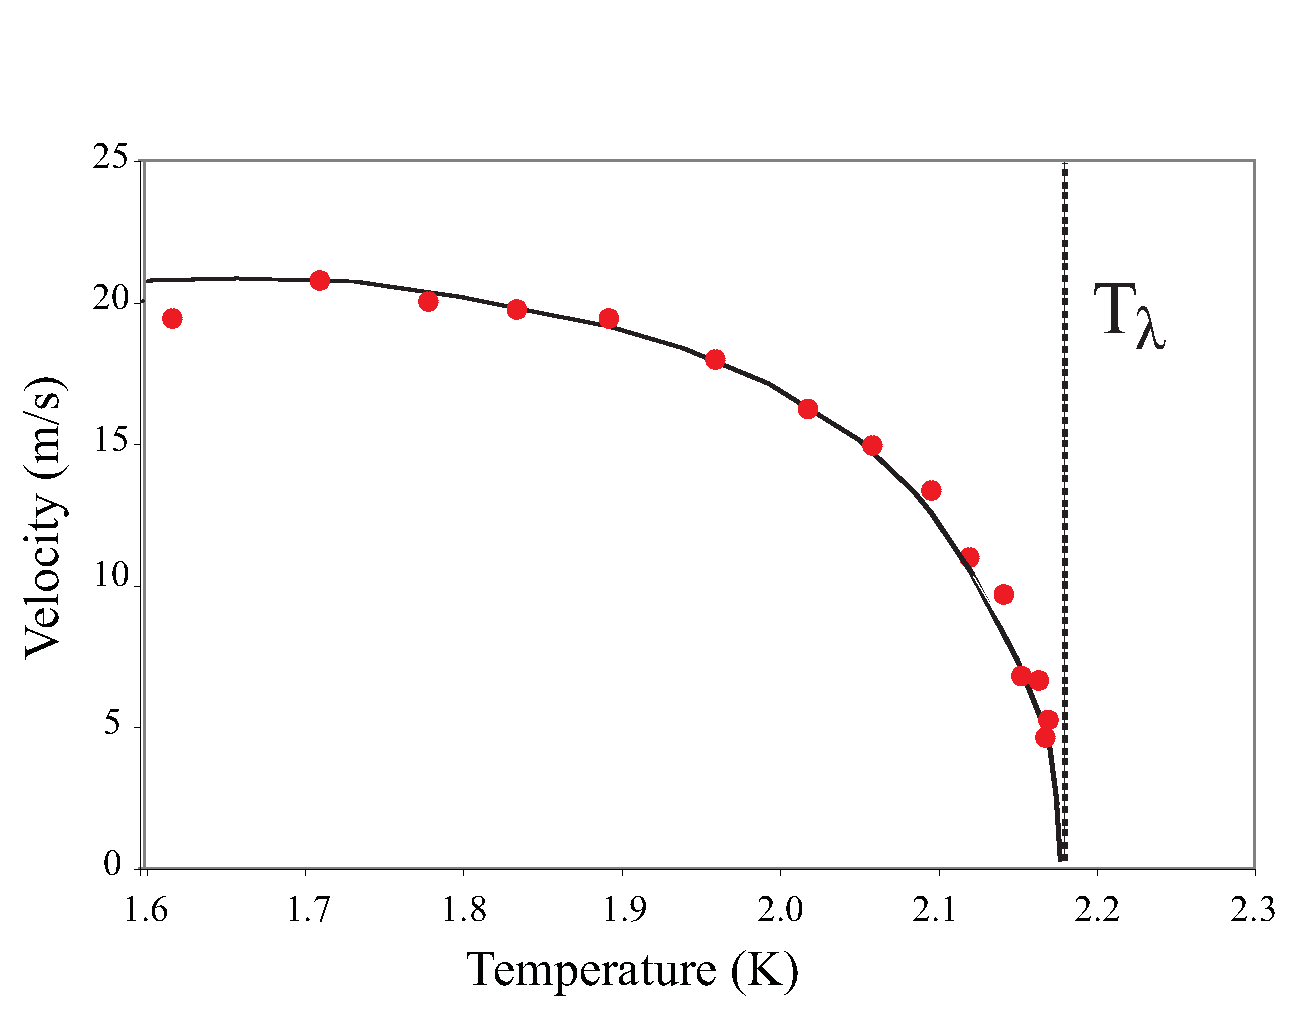
\includegraphics[height=70mm]{./figures/secondsound.eps}
\caption{\small{A plot of the second sound velocity verses temperature in He (II).  This data is compared to Peshkov's results. Second sound velocity goes to zero at the transition from He (II) to He (I) enabling a rough estimate of $T_{\lambda}$.}}
\label{fig:secondsound}
\end{center}
\end{figure}

%\footnote{V. Peshkov, "'Second Sound' in Helium II," J. Phys. (Moscow) 8, 381 (1944)}

\subsection{Heat Capacity Analysis}\label{heatcapacityanalysis}
\subsubsection{Temperature Calibration}\label{temperaturecalibration}

\begin{figure}[htbp]
\begin{center}
\includegraphics[height=70mm]{./figures/.eps}
\caption{\small{}}
\label{fig:}
\end{center}
\end{figure}

\subsubsection{Calculating the Heat Capacity of the Cell}\label{calculatingtheheatcapacityofthecell}

\begin{figure}[htbp]
\begin{center}
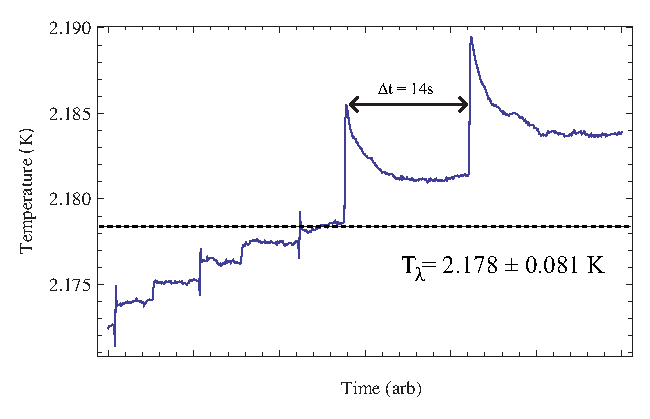
\includegraphics[height=70mm]{./figures/heatingdata.eps}
\caption{\small{A plot of the data from Figure~\ref{fig:rawdata} (b) after being converted from electric potential to temperature using the calibration in \ref{temperaturecalibration}.  From this data, $T_{\lambda}$ is determined to be $2.176\pm0.010$ K.}}
\label{fig:heatingdata}
\end{center}
\end{figure}

\begin{figure}[htbp]
\begin{center}
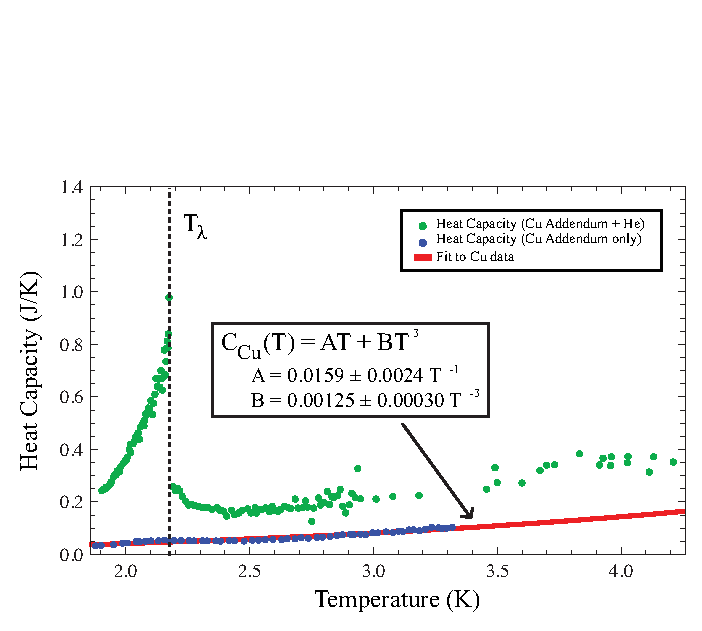
\includegraphics[height=70mm]{./figures/lambdanorm.eps}
\caption{\small{A plot of the heat capacity of the Cu addendum filled with He (II)) and the heat capacity of the evacuated Cu addendum.  A polynomial with cubic and linear terms was fit to the Cu data in order to ultimately remove the addendum's contribution to the heat capacity data.}}
\label{fig:lambdanorm}
\end{center}
\end{figure}

\subsubsection{Calculating the Specific Heat of Superfluid Helium}\label{calculatingthespecificheatofsuperfluidhelium}

\begin{figure}[htbp]
\begin{center}
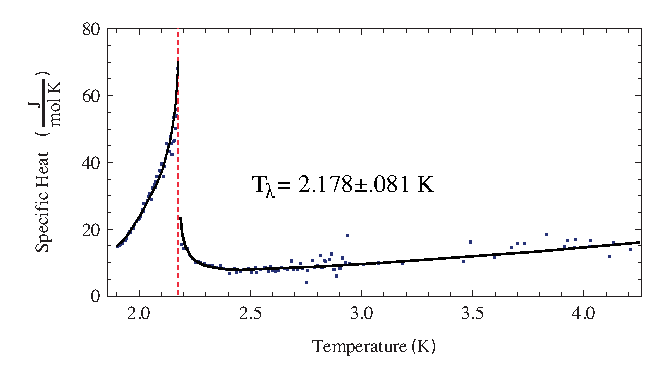
\includegraphics[height=70mm]{./figures/lambdatrans.eps}
\caption{\small{A plot of the specific heat of He(II) verses temperature. The transition from He(I) to He (II) occurs at $T_{\lambda} = 2.176 \pm .010$ K.  The values for specific heat each have a statistical error of $Blah$ J/mol K.}}
\label{fig:lambdatrans}
\end{center}
\end{figure}

